%
% tikztemplate.tex
%
% (c) 2018 Prof Dr Andreas Müller, Hochschule Rapperswil
%
\documentclass[tikz]{standalone}
\usepackage{times}
\usepackage{amsmath}
\usepackage{txfonts}
\usepackage[utf8]{inputenc}
\usepackage{graphics}
\usepackage{color}
\usepackage{pifont}
\usetikzlibrary{arrows,intersections,math,calc}
\begin{document}

\def\punkt#1{
        \fill[color=white] #1 circle[radius=0.08];
        \draw #1 circle[radius=0.08];
}

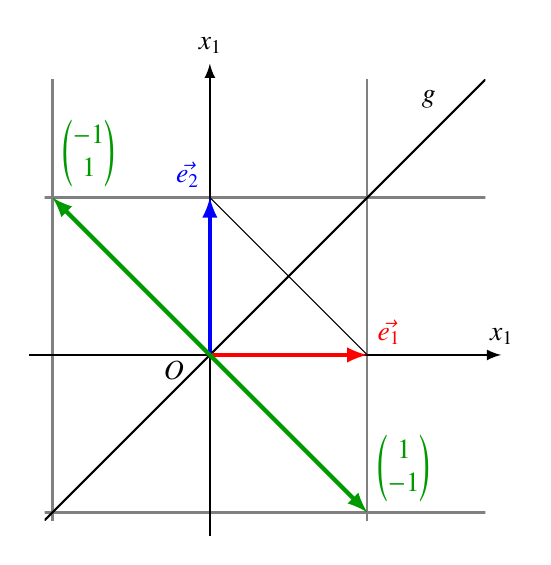
\begin{tikzpicture}[>=latex,thick]

\coordinate (O) at (0,0);
\coordinate (A) at (6,6);
\coordinate (B) at (-6,-6);

\begin{scope}
\clip (-2.1,-2.1) rectangle (3.5,3.5);
\draw[color=gray,step=2] (A) grid (B);
\draw (A) to (B);
\end{scope}

\draw[line width=0.4pt] (2,0)--(0,2);

\draw[->] (-2.3,0)--(3.7,0) coordinate[label={$x_1$}];
\draw[->] (0,-2.3)--(0,3.7) coordinate[label={$x_1$}];

\draw[->,line width=1.5pt,color=red] (O)--(2,0);
\node[color=red] at (2,0) [above right] {$\vec{e_1}$};
\draw[->,line width=1.5pt,color=blue] (O)--(0,2);
\node[color=blue] at (0,2) [above left] {$\vec{e_2}$};

\node at (3,3) [above left] {$g$};

\definecolor{darkgreen}{rgb}{0,0.6,0}

\draw[->,line width=1.5pt,color=darkgreen] (0,0)--(2,-2);
\draw[->,line width=1.5pt,color=darkgreen] (0,0)--(-2,2);
\node[color=darkgreen] at (2,-2) [above right] {$\begin{pmatrix}1\\-1\end{pmatrix}$};
\node[color=darkgreen] at (-2,2) [above right] {$\begin{pmatrix}-1\\1\end{pmatrix}$};

\punkt{(O)} \node at (-0.2,0.05) [below left] {$O$};

\end{tikzpicture}

\end{document}

